%% thesis.tex -- stress test for utad-tfg.cls. FILLER ONLY.
%%
%% Every paragraph is lipsum / kantlipsum pseudo-prose or a public-domain
%% passage (Cervantes 1605, Darwin 1859) and every number is synthetic.
%% Nothing here is thesis text.
%%
%% Build (both languages):   ./build.sh
%% One language:             latexmk -pdf -usepretex -pretex='\def\tfglang{spanish}' -jobname=thesis-es thesis.tex

\ifdefined\tfglang\else\def\tfglang{english}\fi
\expandafter\documentclass\expandafter[\tfglang]{utad-tfg}

\usepackage[style=apa,backend=biber]{biblatex}
\addbibresource{refs.bib}
% biblatex prints URLs with its own breaking rules, not xurl's: by default
% it breaks only at punctuation, and a 36-letter path segment ran 16pt
% into the margin in the Spanish build. These allow breaks between letters.
\setcounter{biburlnumpenalty}{9000}
\setcounter{biburlucpenalty}{9000}
\setcounter{biburllcpenalty}{9000}
\usepackage{lipsum}
\usepackage{kantlipsum}
\usepackage{longtable}
\usepackage{listings}
\lstset{basicstyle=\ttfamily\small, breaklines=true, frame=single,
  columns=fullflexible, keepspaces=true, showstringspaces=false}
% listings numbers per chapter ("Listing 3.1") where the class numbers
% figures and tables continuously; make it match.
\AtBeginDocument{\counterwithout{lstlisting}{chapter}}
\graphicspath{{figures/}}

% ---- Cover ---------------------------------------------------------
\tfgtitle{A stress test of the utad-tfg class with seventy pages of filler}
\tfgmodality{conventional}
\tfgdegree{DEGREE IN SOFTWARE ENGINEERING, SPECIALIZATION IN NOTHING IN PARTICULAR}
\tfgcall{ORDINARY, ACADEMIC YEAR 2026--2027}
\tfgstudent{TEST STUDENT SURNAME SURNAME}
\tfgtutor{TEST TUTOR SURNAME}
\tfgcotutor{}

\begin{document}

\tfgcover

\begin{tfgacknowledgements}
\lipsum[1]
\end{tfgacknowledgements}

\textit{This is the style note page. The index follows on this page, as in
the template, and runs onto the next.}

\tfgindex

\begin{tfgabstractpage}
\tfgabstract{\lipsum[2]}{filler, test, stress, class, index}
\tfgaltabstract{\lipsum[3]}{relleno, prueba, clase, índice}
\end{tfgabstractpage}

% =====================================================================
\chapter{Introduction}
\label{ch:intro}

\lipsum[4-5]

\section{Justification and context}
\label{sec:context}
\lipsum[6-7] This sentence carries a footnote.\footnote{A footnote with
enough text to wrap onto a second line, so that the footnote leading and
the rule above it can be inspected; \lipsum[66]} And this one carries
another.\footnote{Second footnote on the same page.}

\lipsum[8]

\section{Motivation}
\kant[1-2]

\section{Problem statement}
The long quotation below is the closing sentence of \textcite{darwin1859},
public domain, set in the template's Quote style:
\begin{tfgquote}
There is grandeur in this view of life, with its several powers, having been
originally breathed into a few forms or into one; and that, whilst this
planet has gone cycling on according to the fixed law of gravity, from so
simple a beginning endless forms most beautiful and most wonderful have
been, and are being, evolved.
\end{tfgquote}
\lipsum[9-10]

\section{Objectives}
\begin{enumerate}
  \item General objective: \lipsum[11][1-2]
  \item Specific objective one: see Chapter~\ref{ch:dev}, Section~\ref{sec:deep},
        Figure~\ref{fig:wide} and Table~\ref{tab:long}.
  \item Specific objective two: \lipsum[11][3-4]
\end{enumerate}
\lipsum[12-13]

% =====================================================================
\chapter{State of the art}
\label{ch:sota}

\lipsum[14-15] \parencite{knuth1984,lamport1994,mittelbach2004}.

\section{First area}
\lipsum[16-17] \textcite{codd1970} and \textcite{turing1936} are cited here
only to exercise the citation machinery \parencite{shannon1948,dijkstra1968}.

\begin{figure}[htbp]
  \centering
  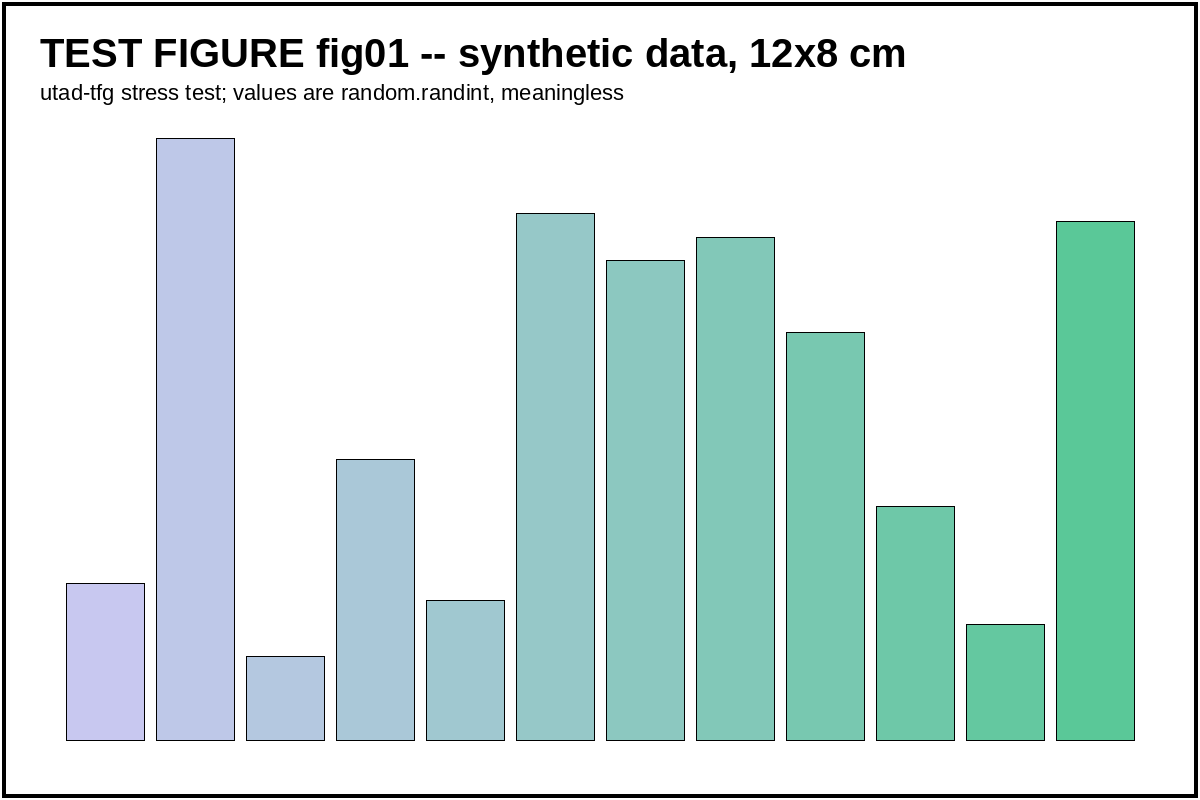
\includegraphics[width=12cm]{fig01}
  \caption{First test figure. \source{Synthetic, generated by the test script (2026)}}
  \label{fig:one}
\end{figure}

\subsection{First subsection}
\lipsum[18-19]

\subsubsection{First sub-subsection}
\lipsum[20]

\paragraph{Fourth level}
\lipsum[21][1-3]

\subparagraph{Fifth level below the chapter}
\lipsum[21][4-6] This heading is numbered
\ref{ch:sota}.1.1.1.1.1 if secnumdepth is 5.

\subsection{Second subsection}
\lipsum[22-23]

\begin{figure}[htbp]
  \centering
  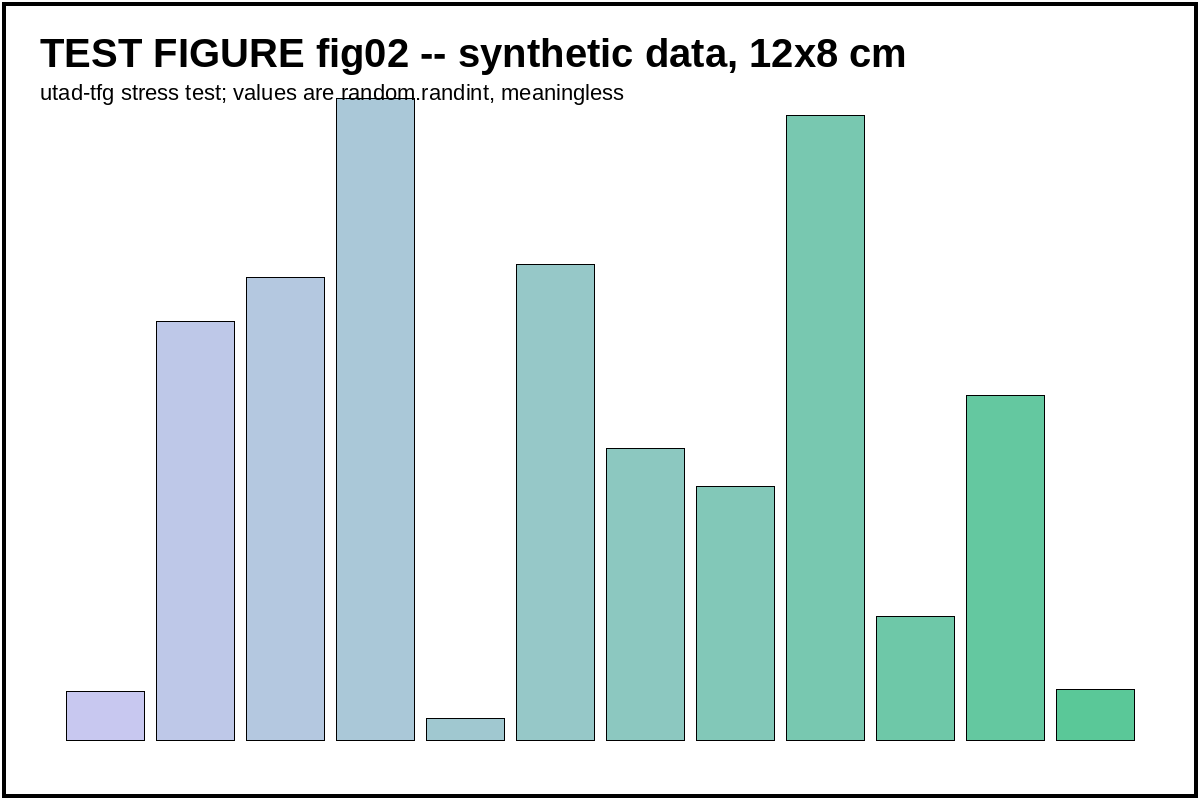
\includegraphics[width=12cm]{fig02}
  \caption{Second test figure, placed with htbp. \source{Synthetic (2026)}}
  \label{fig:two}
\end{figure}

\section{Second area}
\lipsum[24-25] \parencite{brooks1975,knuth1997,kernighan1988,gamma1994,cormen2009}.

\begin{table}[htbp]
  \centering
  \caption{A short booktabs table. \source{Synthetic (2026)}}
  \label{tab:short}
  \begin{tabular}{lrr}
    \toprule
    Item & Value & Unit \\
    \midrule
    alpha & 1.0 & ms \\
    beta  & 22.5 & ms \\
    gamma & 333.25 & ms \\
    \bottomrule
  \end{tabular}
\end{table}

\lipsum[26-28]

\section{Third area}
\kant[3-5]

\begin{figure}[htbp]
  \centering
  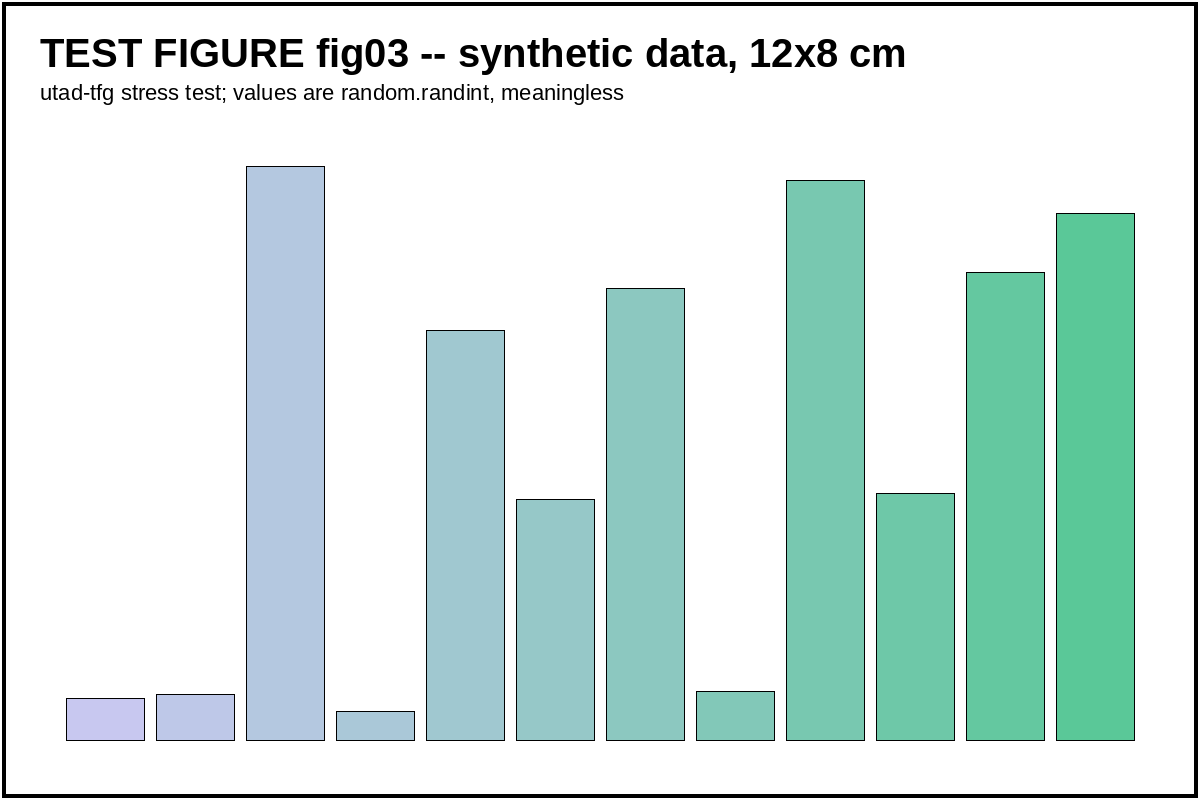
\includegraphics[width=12cm]{fig03}
  \caption{Third test figure. \source{Synthetic (2026)}}
  \label{fig:three}
\end{figure}

\lipsum[29-31] \parencite{bernerslee1994,knuthplass1981,vaswani2017}.

\section{Fourth area, with a public-domain Spanish passage}
The following paragraphs are the opening of \textcite{cervantes1605},
public domain, included so that Spanish hyphenation can be checked in the
[spanish] build:

En un lugar de la Mancha, de cuyo nombre no quiero acordarme, no ha mucho
tiempo que vivía un hidalgo de los de lanza en astillero, adarga antigua,
rocín flaco y galgo corredor. Una olla de algo más vaca que carnero,
salpicón las más noches, duelos y quebrantos los sábados, lantejas los
viernes, algún palomino de añadidura los domingos, consumían las tres
partes de su hacienda. El resto della concluían sayo de velarte, calzas de
velludo para las fiestas, con sus pantuflos de lo mesmo, y los días de
entresemana se honraba con su vellorí de lo más fino. Tenía en su casa una
ama que pasaba de los cuarenta y una sobrina que no llegaba a los veinte, y
un mozo de campo y plaza que así ensillaba el rocín como tomaba la
podadera. Frisaba la edad de nuestro hidalgo con los cincuenta años. Era de
complexión recia, seco de carnes, enjuto de rostro, gran madrugador y amigo
de la caza. Quieren decir que tenía el sobrenombre de Quijada, o Quesada,
que en esto hay alguna diferencia en los autores que deste caso escriben,
aunque por conjeturas verisímiles se deja entender que se llamaba Quijana.
Pero esto importa poco a nuestro cuento: basta que en la narración dél no
se salga un punto de la verdad.

Es, pues, de saber que este sobredicho hidalgo, los ratos que estaba
ocioso, que eran los más del año, se daba a leer libros de caballerías, con
tanta afición y gusto, que olvidó casi de todo punto el ejercicio de la
caza y aun la administración de su hacienda; y llegó a tanto su curiosidad
y desatino en esto, que vendió muchas hanegas de tierra de sembradura para
comprar libros de caballerías en que leer, y así, llevó a su casa todos
cuantos pudo haber dellos; y de todos, ningunos le parecían tan bien como
los que compuso el famoso Feliciano de Silva, porque la claridad de su prosa
y aquellas entricadas razones suyas le parecían de perlas, y más cuando
llegaba a leer aquellos requiebros y cartas de desafíos, donde en muchas
partes hallaba escrito: La razón de la sinrazón que a mi razón se hace, de
tal manera mi razón enflaquece, que con razón me quejo de la vuestra
fermosura.

\lipsum[32-35]

\begin{figure}[htbp]
  \centering
  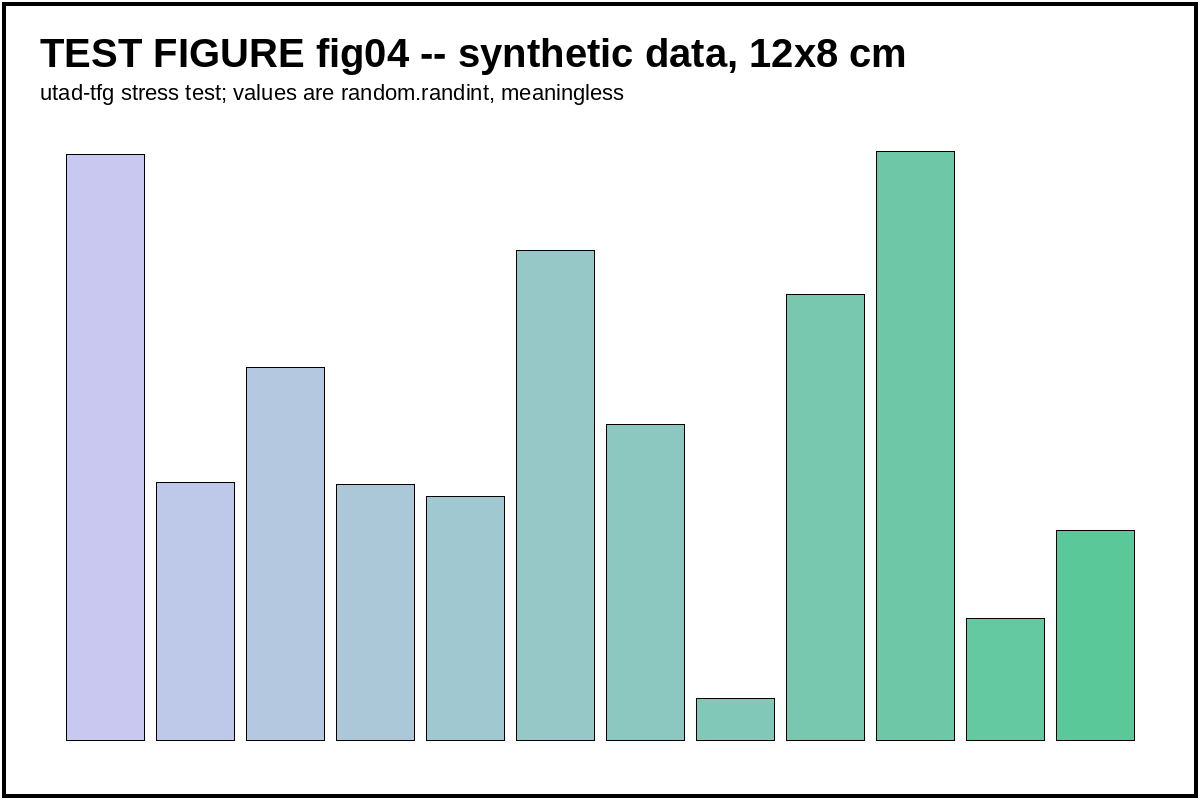
\includegraphics[width=12cm]{fig04}
  \caption{Fourth test figure. \source{Synthetic (2026)}}
  \label{fig:four}
\end{figure}

\lipsum[36-38]

% =====================================================================
\chapter{Methodology}
\label{ch:method}

\lipsum[39-40] \parencite{hevner2004,peffers2007,wieringa2014}.

\section{Tables}
Table~\ref{tab:short} on page~\pageref{tab:short} was short. Table~\ref{tab:long}
spans pages. Table~\ref{tab:wide} fills the text width.

\begin{table}[htbp]
  \centering
  \caption{A table filling the text width with tabularx-free fixed columns. \source{Synthetic (2026)}}
  \label{tab:wide}
  \begin{tabular}{p{3cm}p{3cm}p{3cm}p{3.5cm}}
    \toprule
    Column one & Column two & Column three & Column four \\
    \midrule
    \lipsum[1][1] & \lipsum[2][1] & \lipsum[3][1] & \lipsum[4][1] \\
    short & short & short & short \\
    \bottomrule
  \end{tabular}
\end{table}

\lipsum[41]

\begin{longtable}{rllr}
  \caption{A longtable that spans pages; 70 synthetic rows. \source{Synthetic (2026)}}
  \label{tab:long}\\
  \toprule
  Row & Key & Description & Value \\
  \midrule
  \endfirsthead
  \caption[]{(continued)}\\
  \toprule
  Row & Key & Description & Value \\
  \midrule
  \endhead
  \midrule
  \multicolumn{4}{r}{\small continues on the next page}\\
  \endfoot
  \bottomrule
  \endlastfoot
  % 70 synthetic rows for the longtable, generated by build of the stress test
  1 & key-1 & synthetic description text for row 1 & 37 \\
  2 & key-2 & synthetic description text for row 2 & 74 \\
  3 & key-3 & synthetic description text for row 3 & 111 \\
  4 & key-4 & synthetic description text for row 4 & 148 \\
  5 & key-5 & synthetic description text for row 5 & 185 \\
  6 & key-6 & synthetic description text for row 6 & 222 \\
  7 & key-7 & synthetic description text for row 7 & 259 \\
  8 & key-8 & synthetic description text for row 8 & 296 \\
  9 & key-9 & synthetic description text for row 9 & 333 \\
  10 & key-10 & synthetic description text for row 10 & 370 \\
  11 & key-11 & synthetic description text for row 11 & 407 \\
  12 & key-12 & synthetic description text for row 12 & 444 \\
  13 & key-13 & synthetic description text for row 13 & 481 \\
  14 & key-14 & synthetic description text for row 14 & 518 \\
  15 & key-15 & synthetic description text for row 15 & 555 \\
  16 & key-16 & synthetic description text for row 16 & 592 \\
  17 & key-17 & synthetic description text for row 17 & 629 \\
  18 & key-18 & synthetic description text for row 18 & 666 \\
  19 & key-19 & synthetic description text for row 19 & 703 \\
  20 & key-20 & synthetic description text for row 20 & 740 \\
  21 & key-21 & synthetic description text for row 21 & 777 \\
  22 & key-22 & synthetic description text for row 22 & 814 \\
  23 & key-23 & synthetic description text for row 23 & 851 \\
  24 & key-24 & synthetic description text for row 24 & 888 \\
  25 & key-25 & synthetic description text for row 25 & 925 \\
  26 & key-26 & synthetic description text for row 26 & 962 \\
  27 & key-27 & synthetic description text for row 27 & 999 \\
  28 & key-28 & synthetic description text for row 28 & 1036 \\
  29 & key-29 & synthetic description text for row 29 & 1073 \\
  30 & key-30 & synthetic description text for row 30 & 1110 \\
  31 & key-31 & synthetic description text for row 31 & 1147 \\
  32 & key-32 & synthetic description text for row 32 & 1184 \\
  33 & key-33 & synthetic description text for row 33 & 1221 \\
  34 & key-34 & synthetic description text for row 34 & 1258 \\
  35 & key-35 & synthetic description text for row 35 & 1295 \\
  36 & key-36 & synthetic description text for row 36 & 1332 \\
  37 & key-37 & synthetic description text for row 37 & 1369 \\
  38 & key-38 & synthetic description text for row 38 & 1406 \\
  39 & key-39 & synthetic description text for row 39 & 1443 \\
  40 & key-40 & synthetic description text for row 40 & 1480 \\
  41 & key-41 & synthetic description text for row 41 & 1517 \\
  42 & key-42 & synthetic description text for row 42 & 1554 \\
  43 & key-43 & synthetic description text for row 43 & 1591 \\
  44 & key-44 & synthetic description text for row 44 & 1628 \\
  45 & key-45 & synthetic description text for row 45 & 1665 \\
  46 & key-46 & synthetic description text for row 46 & 1702 \\
  47 & key-47 & synthetic description text for row 47 & 1739 \\
  48 & key-48 & synthetic description text for row 48 & 1776 \\
  49 & key-49 & synthetic description text for row 49 & 1813 \\
  50 & key-50 & synthetic description text for row 50 & 1850 \\
  51 & key-51 & synthetic description text for row 51 & 1887 \\
  52 & key-52 & synthetic description text for row 52 & 1924 \\
  53 & key-53 & synthetic description text for row 53 & 1961 \\
  54 & key-54 & synthetic description text for row 54 & 1998 \\
  55 & key-55 & synthetic description text for row 55 & 2035 \\
  56 & key-56 & synthetic description text for row 56 & 2072 \\
  57 & key-57 & synthetic description text for row 57 & 2109 \\
  58 & key-58 & synthetic description text for row 58 & 2146 \\
  59 & key-59 & synthetic description text for row 59 & 2183 \\
  60 & key-60 & synthetic description text for row 60 & 2220 \\
  61 & key-61 & synthetic description text for row 61 & 2257 \\
  62 & key-62 & synthetic description text for row 62 & 2294 \\
  63 & key-63 & synthetic description text for row 63 & 2331 \\
  64 & key-64 & synthetic description text for row 64 & 2368 \\
  65 & key-65 & synthetic description text for row 65 & 2405 \\
  66 & key-66 & synthetic description text for row 66 & 2442 \\
  67 & key-67 & synthetic description text for row 67 & 2479 \\
  68 & key-68 & synthetic description text for row 68 & 2516 \\
  69 & key-69 & synthetic description text for row 69 & 2553 \\
  70 & key-70 & synthetic description text for row 70 & 2590 \\

\end{longtable}

\lipsum[42-43]

\begin{table}[htbp]
  \centering
  \caption{Fourth table. \source{Synthetic (2026)}}
  \label{tab:four}
  \begin{tabular}{lcc}
    \toprule
    Name & A & B \\
    \midrule
    one & 1 & 2 \\
    two & 3 & 4 \\
    \bottomrule
  \end{tabular}
\end{table}

\section{A code listing}
\label{sec:code}
\lipsum[44]

\begin{lstlisting}[language=Python, caption={A test listing (not a thesis artefact).}]
# synthetic script for the utad-tfg stress test; it does nothing useful
def placeholder(values):
    """Return a dictionary of obviously meaningless aggregates."""
    total = sum(values)
    return {"n": len(values), "total": total, "mean": total / max(len(values), 1)}

if __name__ == "__main__":
    print(placeholder([1, 2, 3, 4, 5, 6, 7, 8, 9, 10, 11, 12, 13, 14, 15, 16, 17, 18, 19, 20]))
\end{lstlisting}

\lipsum[45-46]

\section{URLs}
Two long URLs in running text: \url{https://support.microsoft.com/en-us/office/insert-a-table-of-contents-882e8564-0edb-435e-84b5-1d8552ccf0c0}
and \url{https://example.org/another/very/long/placeholder/url/that/has/no/natural/break/points/at/all/abcdefghijklmnopqrstuvwxyz0123456789/end}
\parencite{mstoc,overleaftoc,ctanapa}. \lipsum[47]

\begin{figure}[htbp]
  \centering
  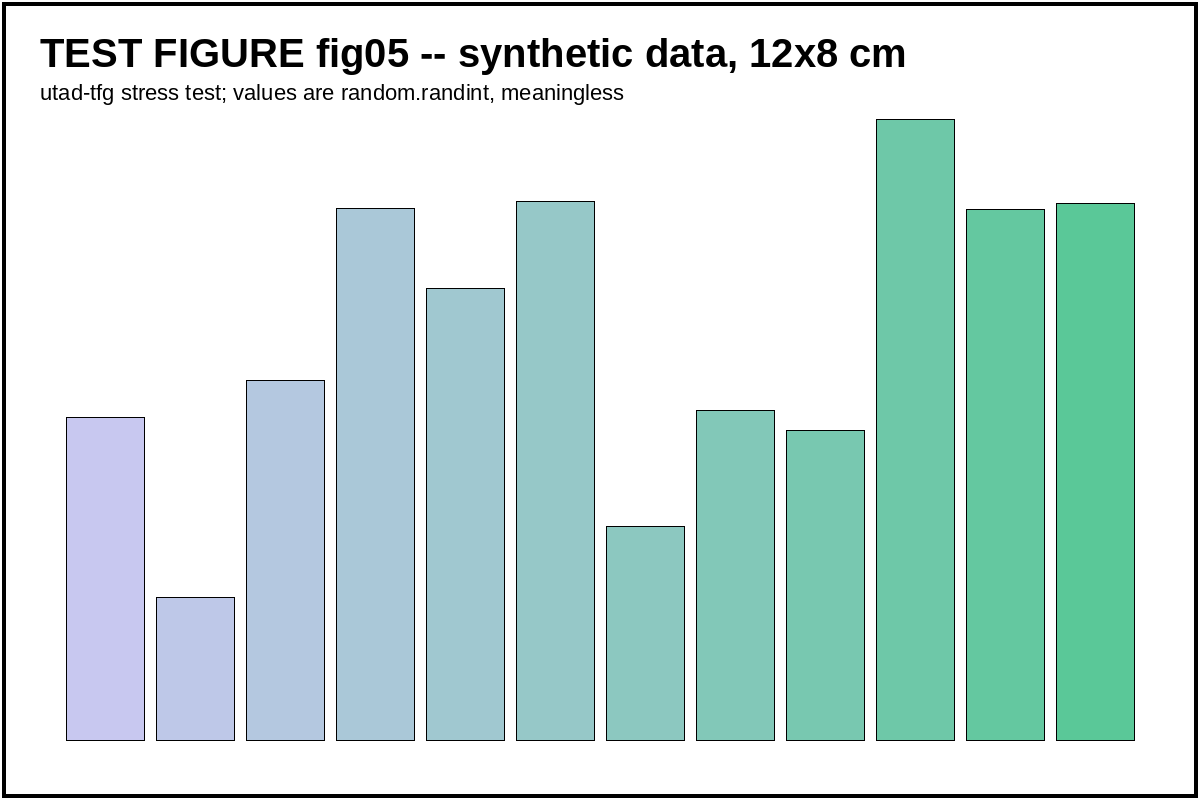
\includegraphics[width=12cm]{fig05}
  \caption{Fifth test figure. \source{Synthetic (2026)}}
  \label{fig:five}
\end{figure}

\lipsum[48-50]

\begin{figure}[htbp]
  \centering
  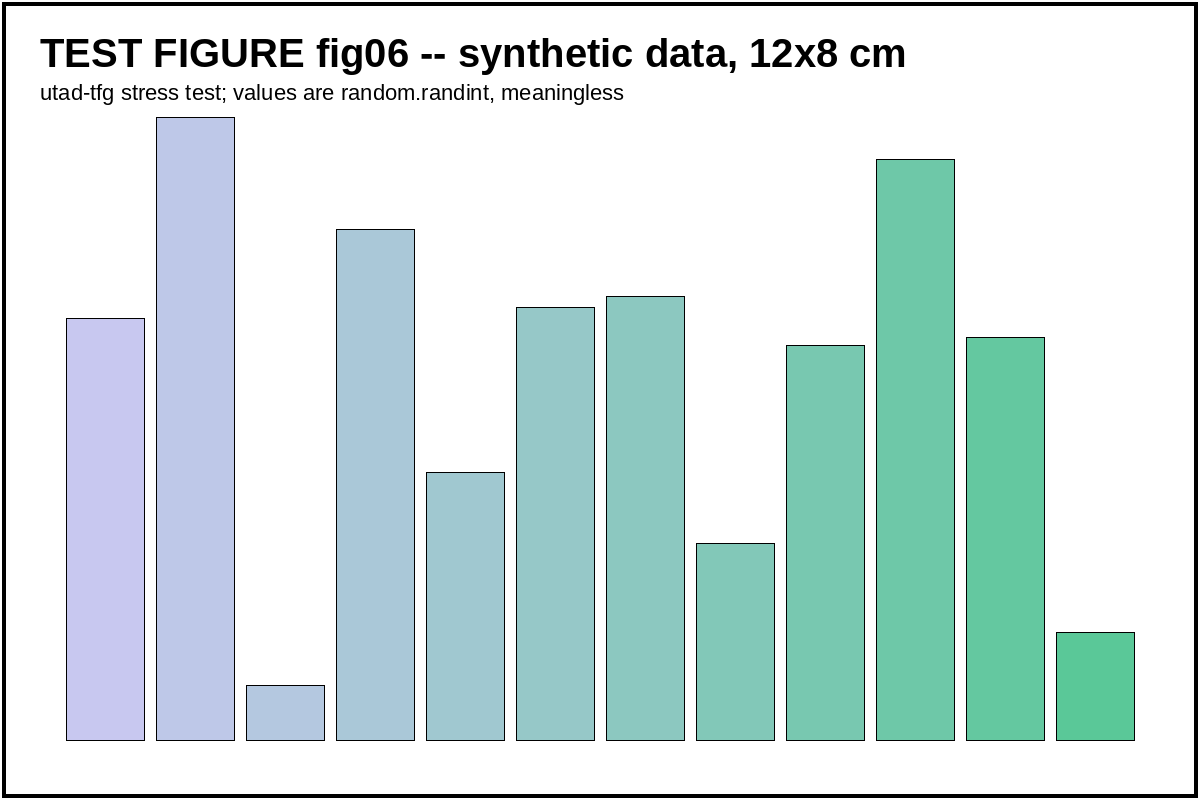
\includegraphics[width=12cm]{fig06}
  \caption{Sixth test figure. \source{Synthetic (2026)}}
\end{figure}

\begin{table}[htbp]
  \centering
  \caption{Fifth table. \source{Synthetic (2026)}}
  \begin{tabular}{ll}
    \toprule
    k & v \\
    \midrule
    a & b \\
    \bottomrule
  \end{tabular}
\end{table}

\section{Employed technologies}
\lipsum[51-53] \parencite{ph01,ph02,ph03,ph04,ph05,ph06,ph07,ph08}.

\begin{figure}[htbp]
  \centering
  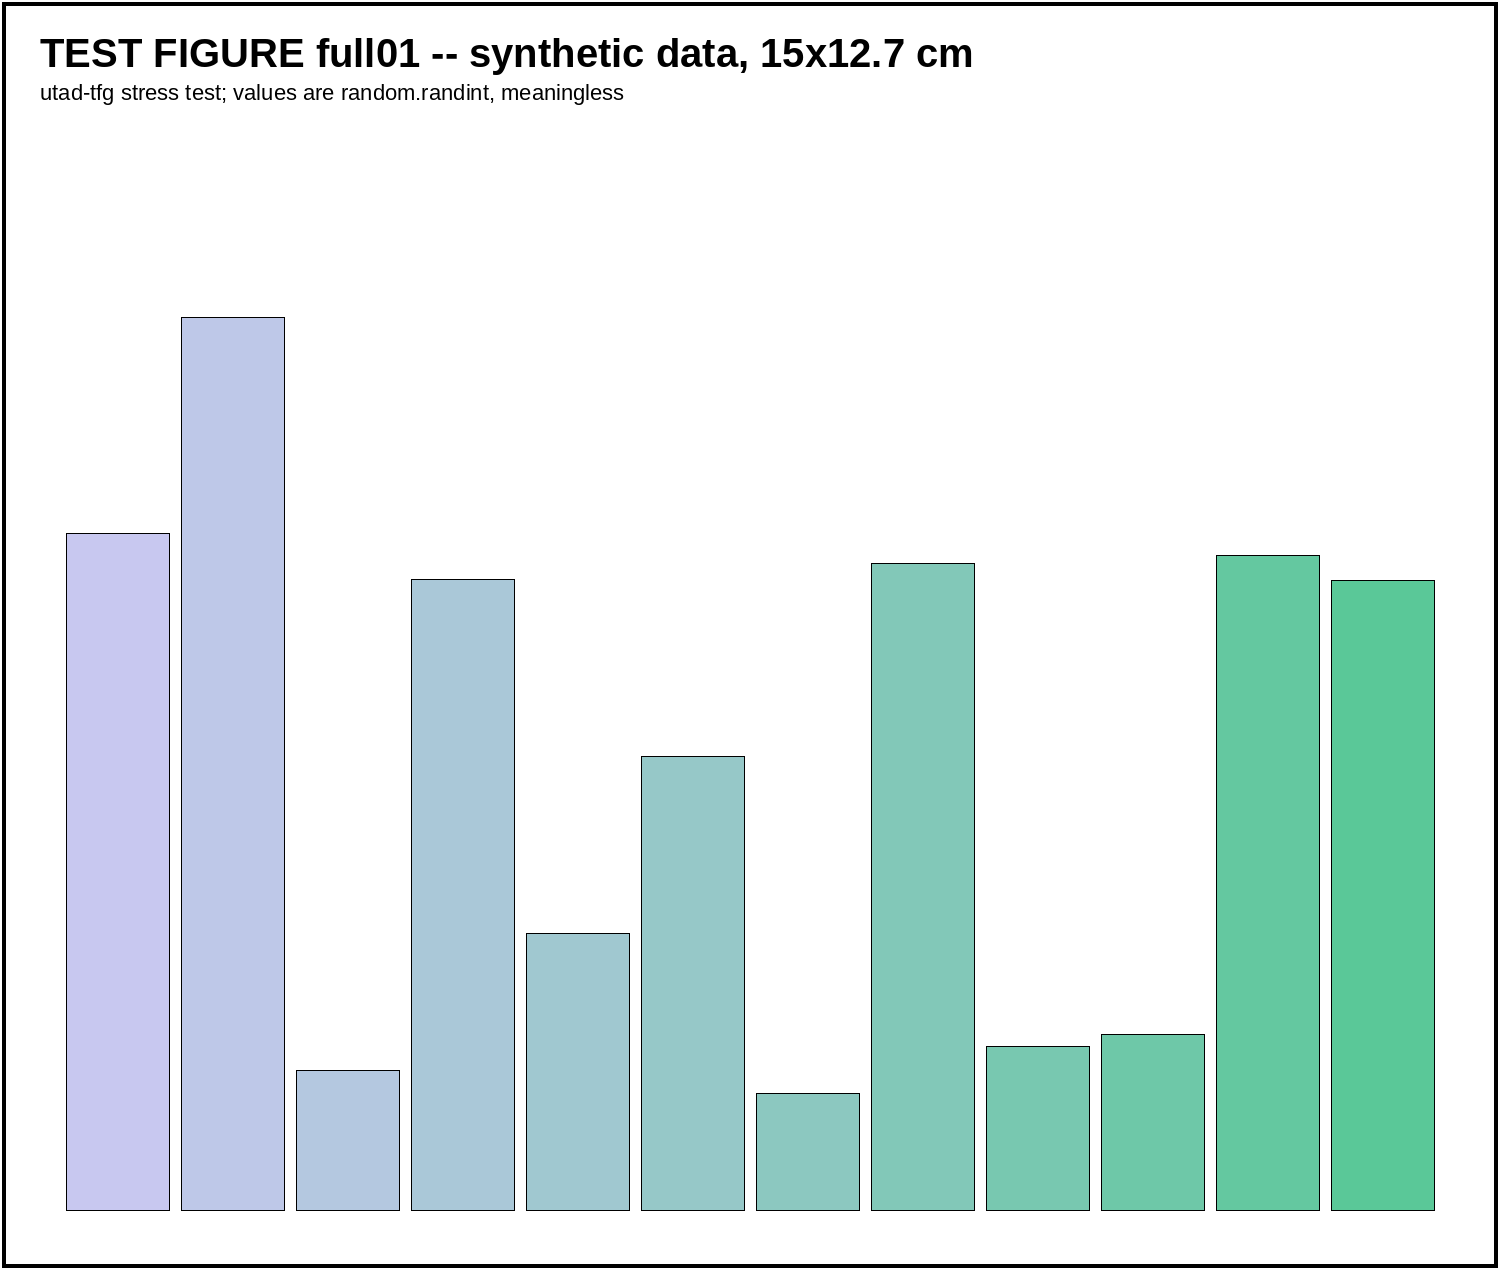
\includegraphics[width=\textwidth]{full01}
  \caption{Seventh test figure, full text width like the template's own. \source{Synthetic (2026)}}
  \label{fig:full}
\end{figure}

\lipsum[54-56]

% =====================================================================
\chapter{Development}
\label{ch:dev}

\lipsum[57-58]

\section{First phase}
\label{sec:deep}
\lipsum[59]

\subsection{Sub}
\lipsum[60]
\subsection{Sub}
\lipsum[61]
\subsection{Sub}
\lipsum[62]
\subsubsection{Subsub}
\lipsum[63]
\subsubsection{Subsub}
\lipsum[64][1-3]
\paragraph{Para}
\lipsum[64][4-6]
\subparagraph{Subpara: numbered 4.1.3.2.1.1}
\label{sec:deepest}
\lipsum[65] Cross-reference back to Section~\ref{sec:context} on
page~\pageref{sec:context} and forward to Figure~\ref{fig:last}.

\begin{figure}[htbp]
  \centering
  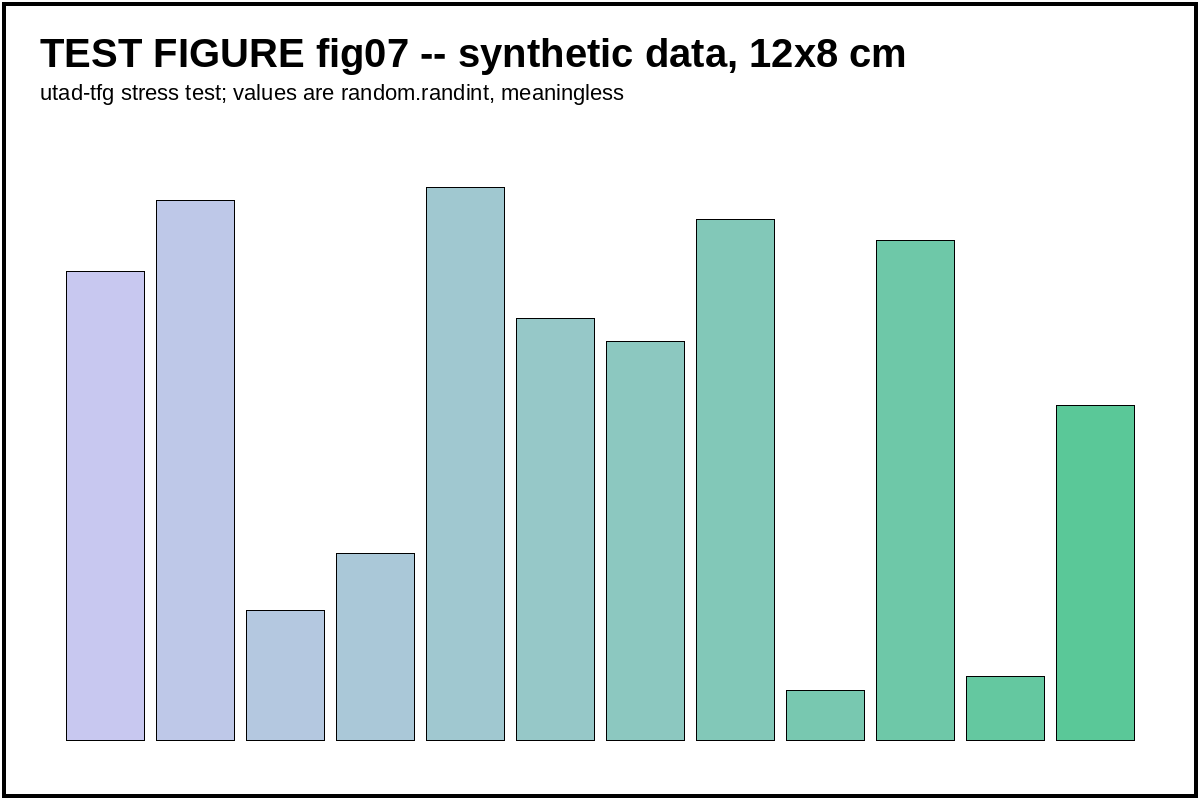
\includegraphics[width=12cm]{fig07}
  \caption{Eighth test figure. \source{Synthetic (2026)}}
\end{figure}

\lipsum[66-68]

\section{A tall figure that forces a page break}
\lipsum[69]
\begin{figure}[htbp]
  \centering
  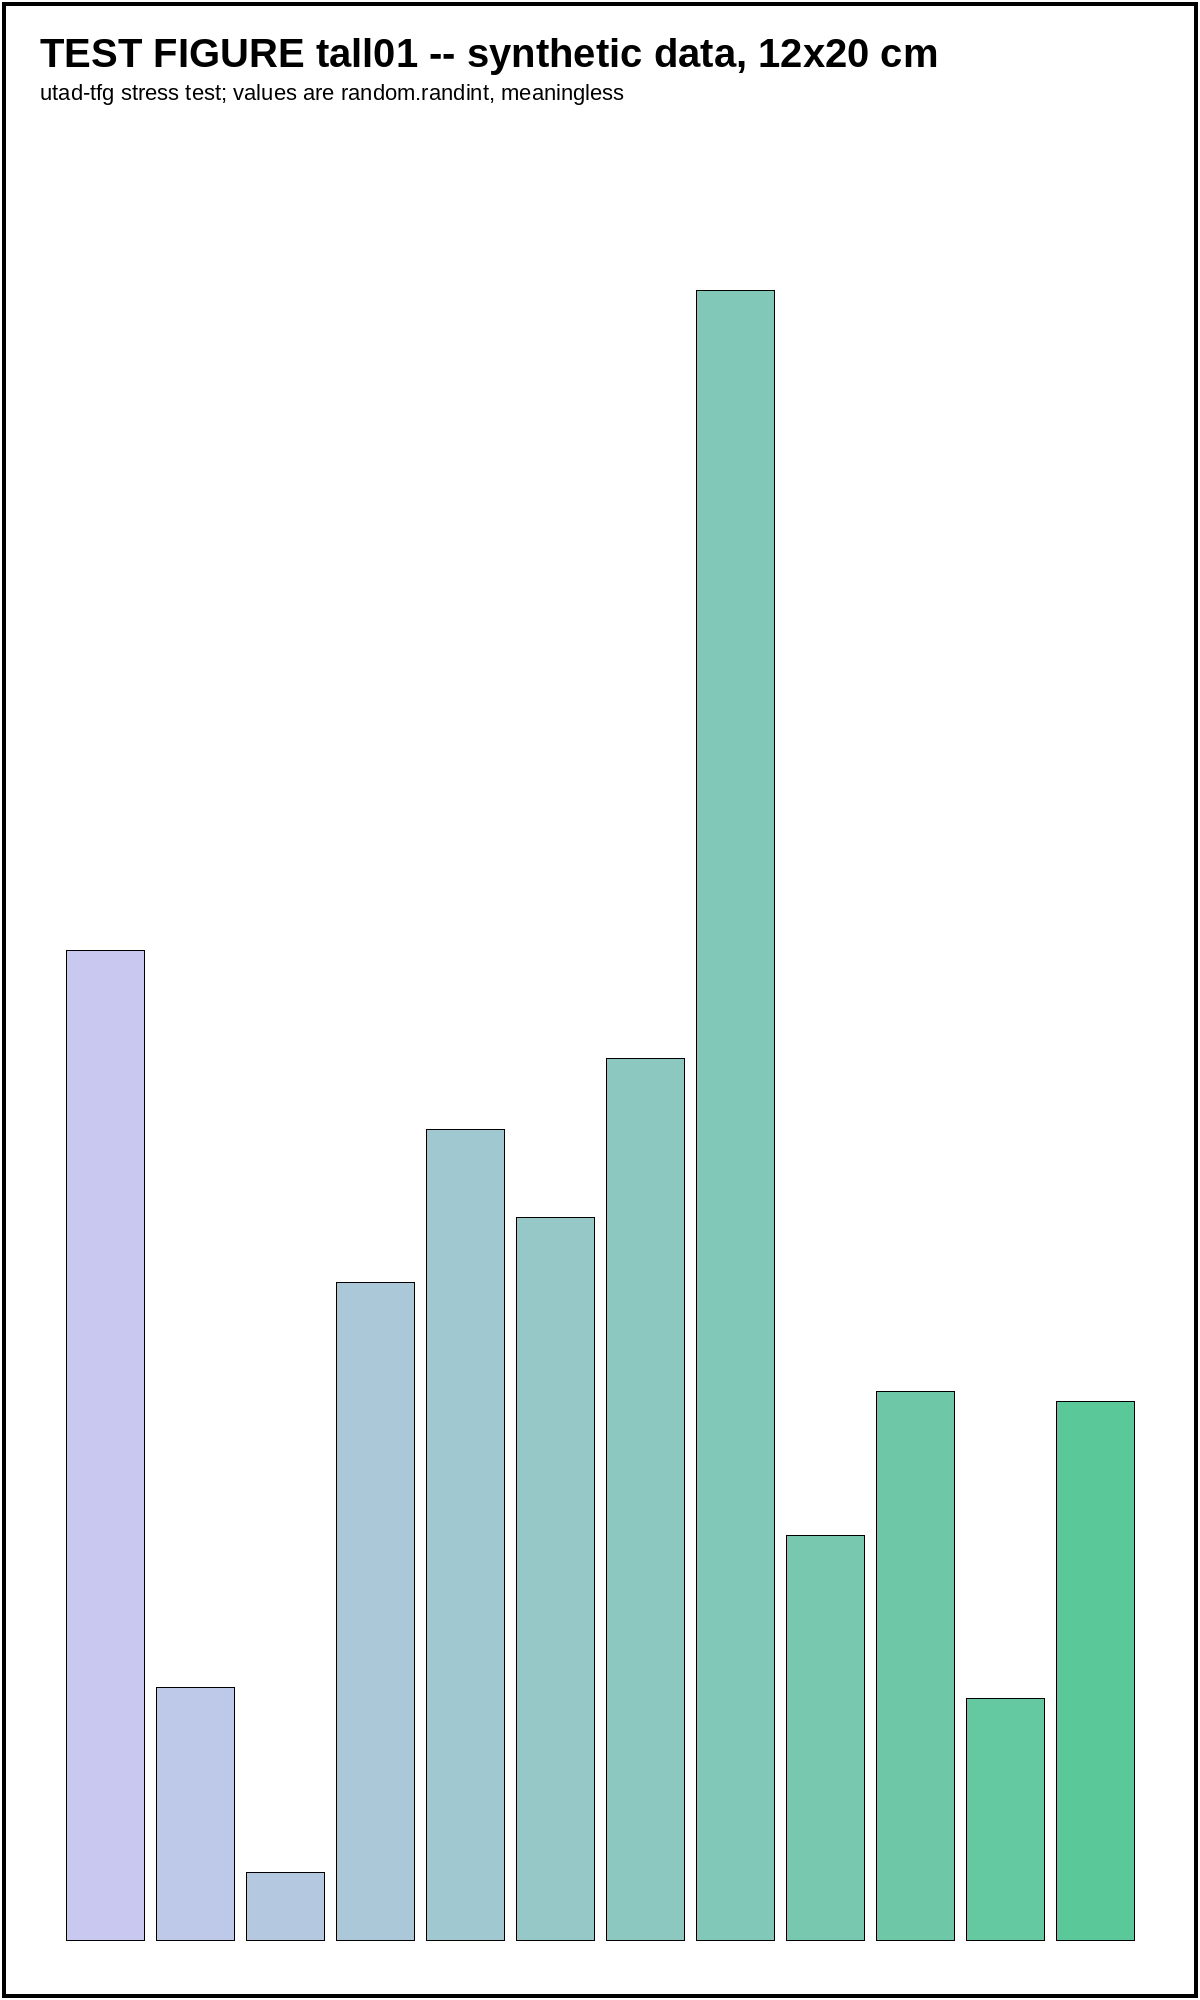
\includegraphics[height=20cm]{tall01}
  \caption{Ninth test figure, 20cm tall. \source{Synthetic (2026)}}
  \label{fig:tall1}
\end{figure}
\lipsum[70-71]

\begin{figure}[p]
  \centering
  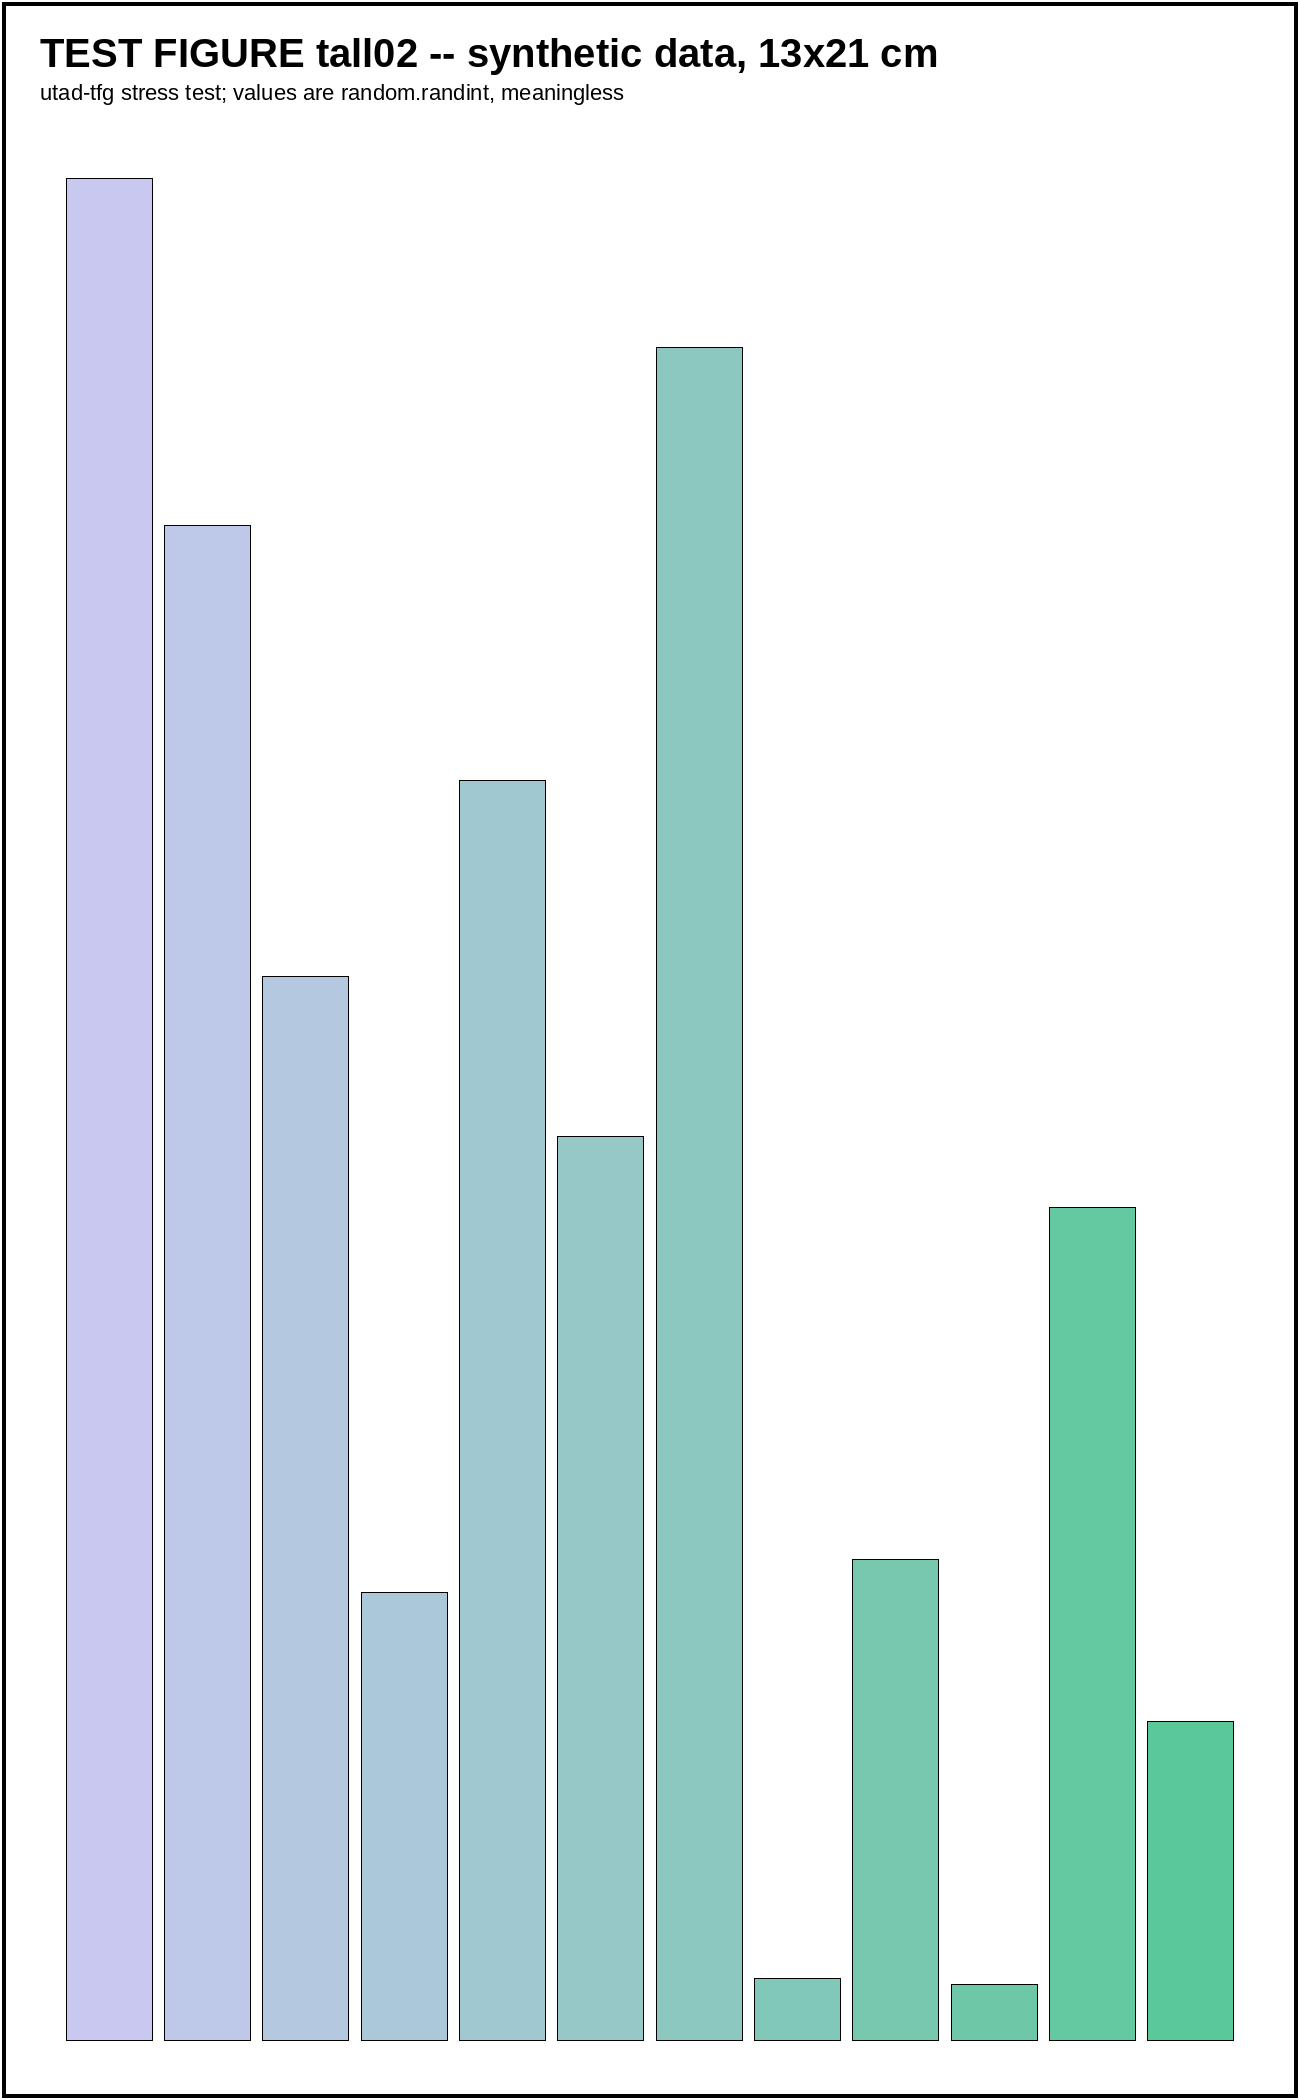
\includegraphics[height=21cm]{tall02}
  \caption{Tenth test figure, 21cm tall, [p]. \source{Synthetic (2026)}}
\end{figure}

\section{A figure wider than the text block}
\lipsum[72]
% 20cm wide against a 15cm text block. Bare, it is an Overfull \hbox of
% 142pt and the image runs off the right edge of the paper (observed).
% \makebox centres the overhang on the text block instead; the class
% itself neither clips nor scales an over-wide box.
\begin{figure}[htbp]
  \centering
  \makebox[\textwidth][c]{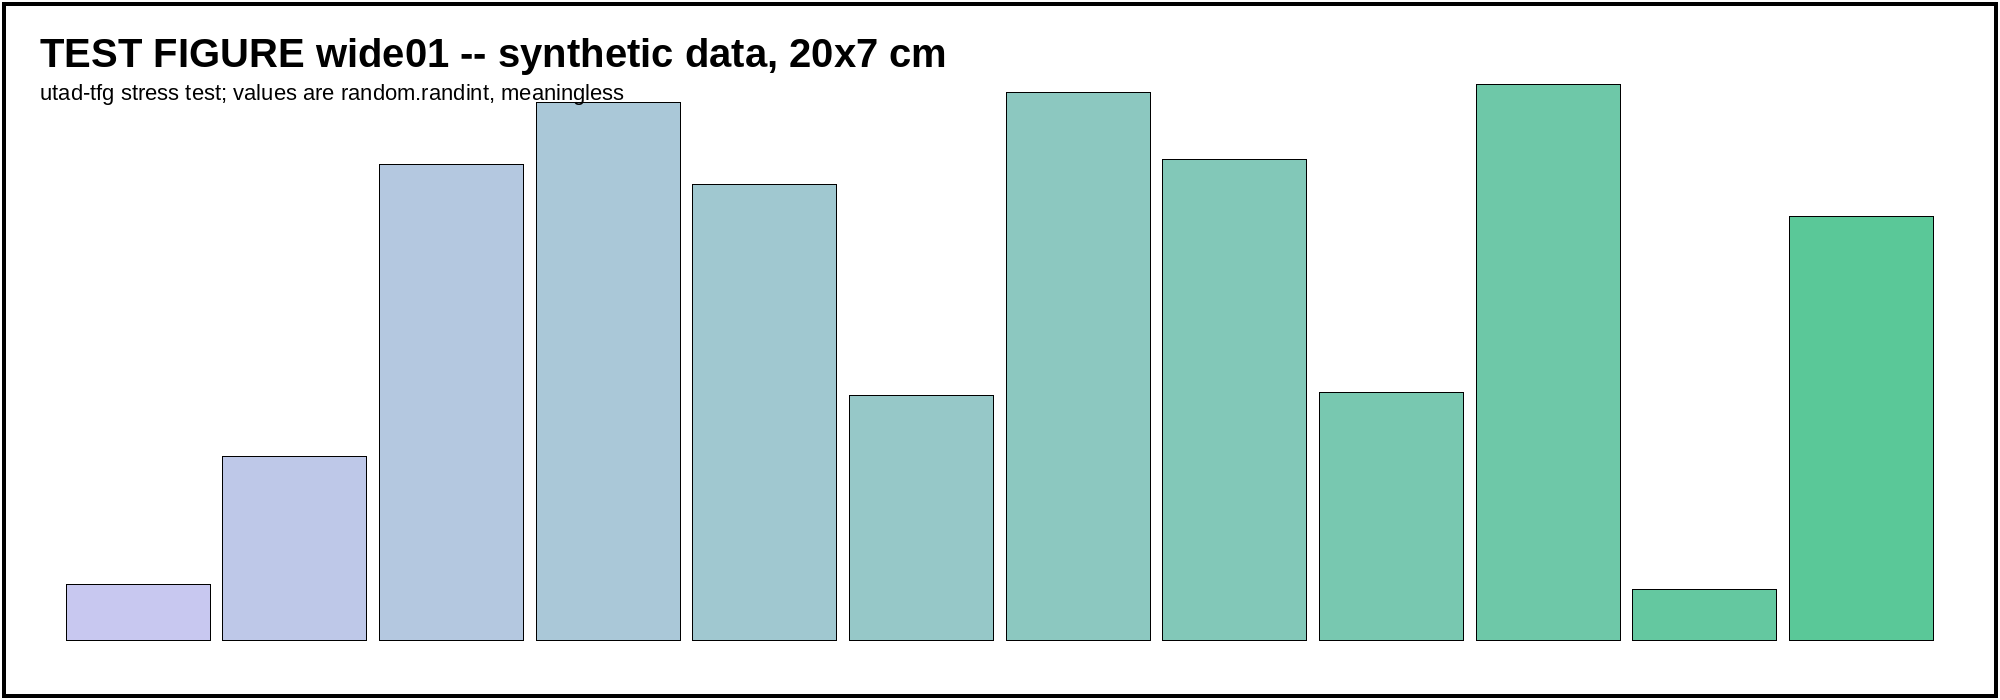
\includegraphics[width=20cm]{wide01}}
  \caption{Eleventh test figure, 20cm wide against a 15cm text block. \source{Synthetic (2026)}}
  \label{fig:wide}
\end{figure}
\lipsum[73-74]

\section{Many figures in a row}
\lipsum[75]
\begin{figure}[htbp]\centering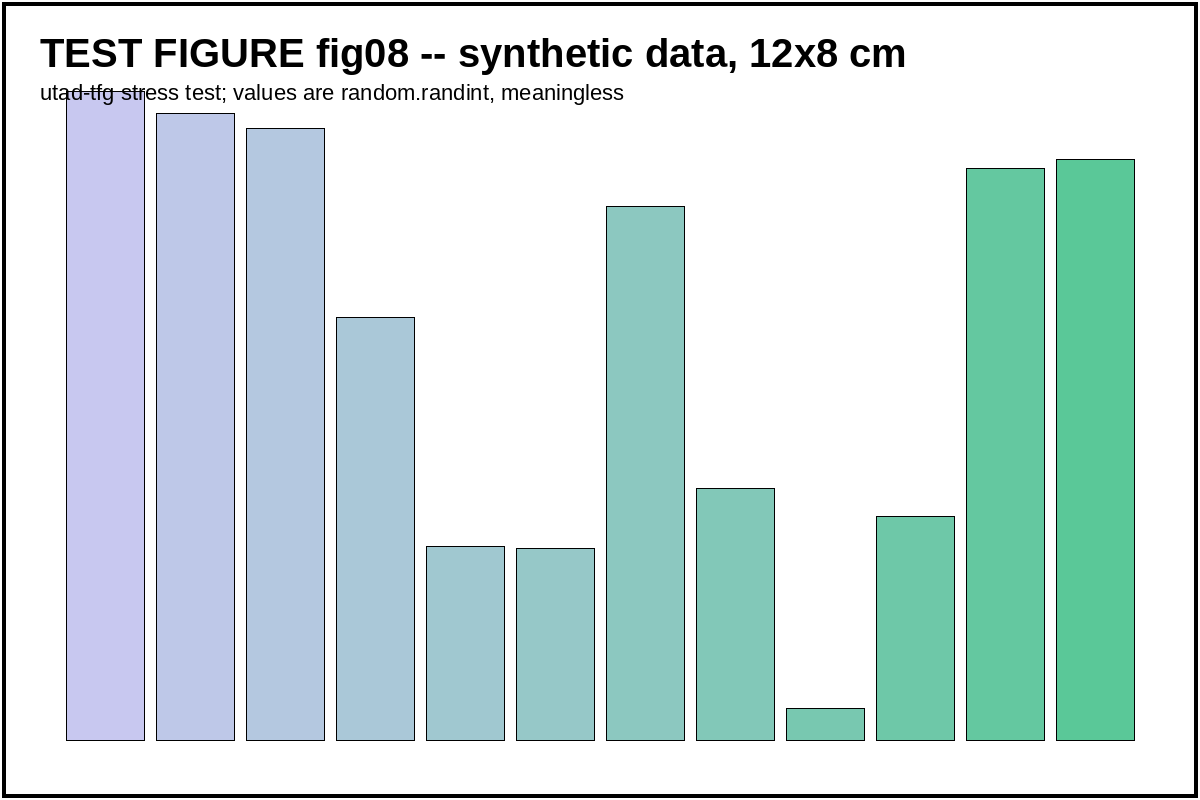
\includegraphics[width=12cm]{fig08}\caption{Twelfth test figure. \source{Synthetic (2026)}}\end{figure}
\begin{figure}[htbp]\centering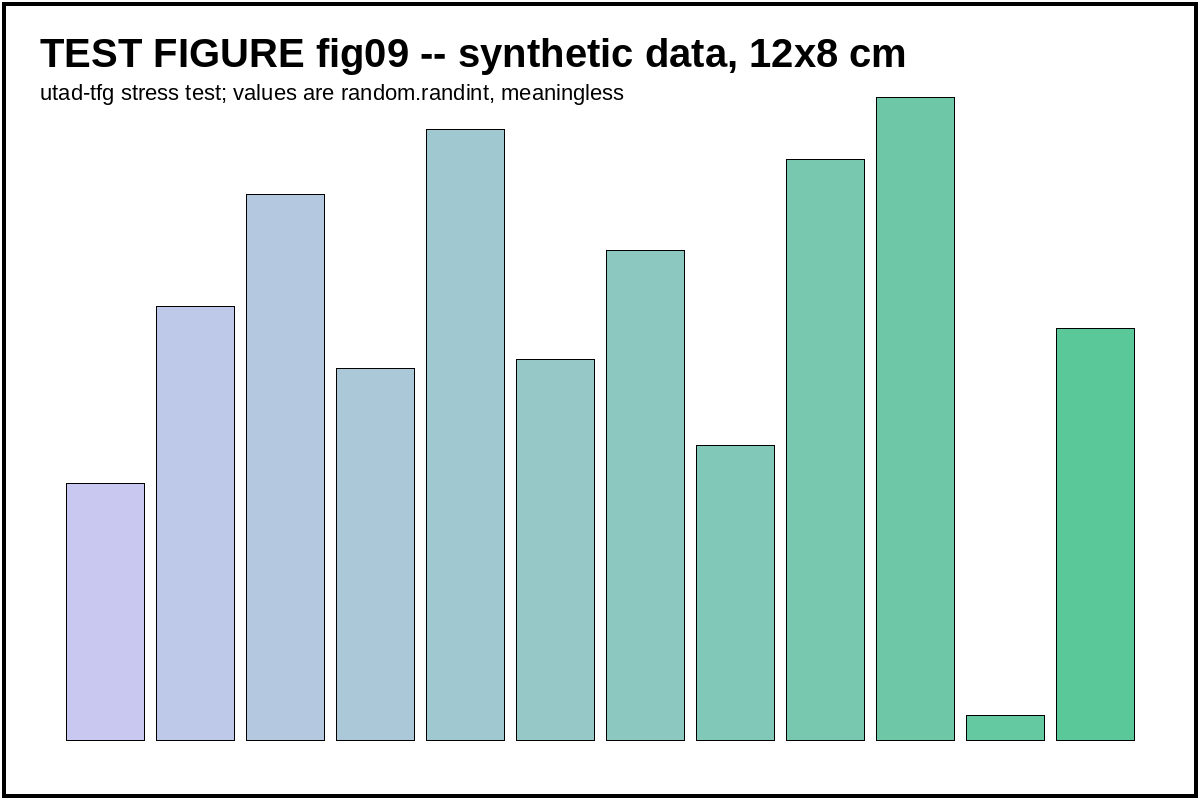
\includegraphics[width=12cm]{fig09}\caption{Thirteenth test figure. \source{Synthetic (2026)}}\end{figure}
\begin{figure}[htbp]\centering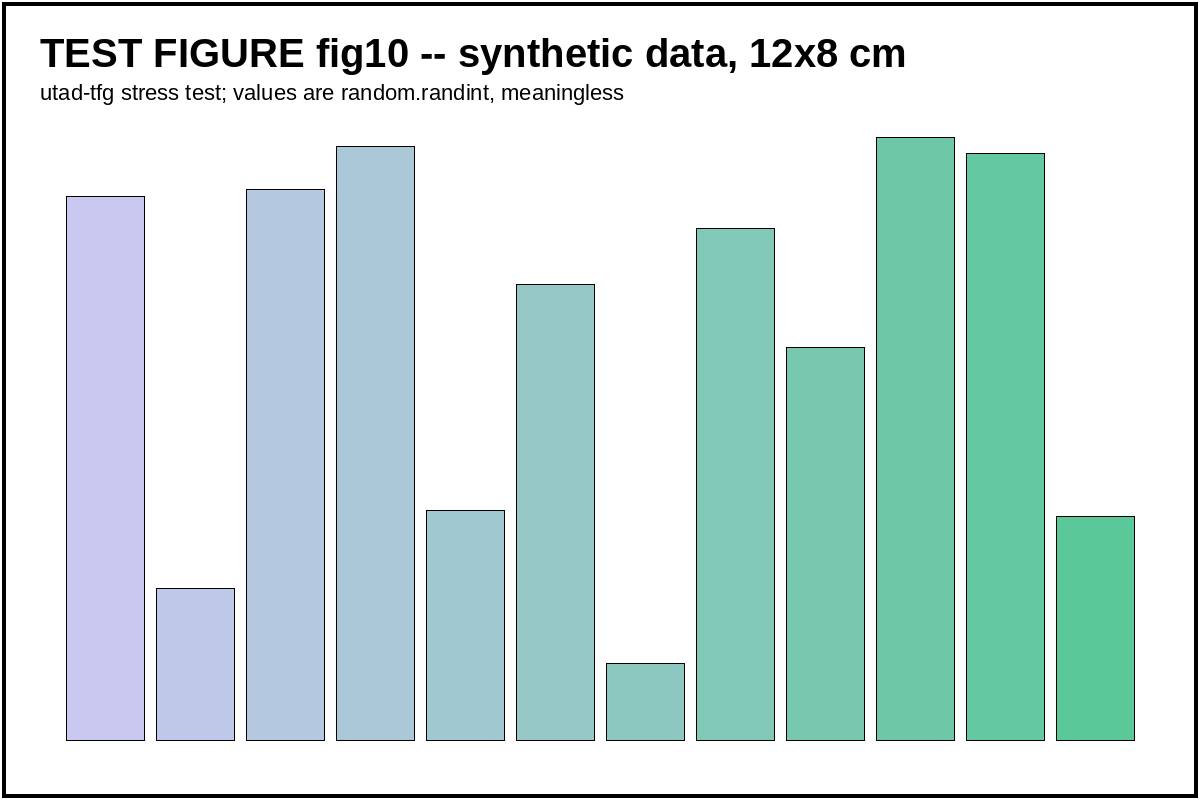
\includegraphics[width=12cm]{fig10}\caption{Fourteenth test figure. \source{Synthetic (2026)}}\end{figure}
\lipsum[76-77]
\begin{figure}[htbp]\centering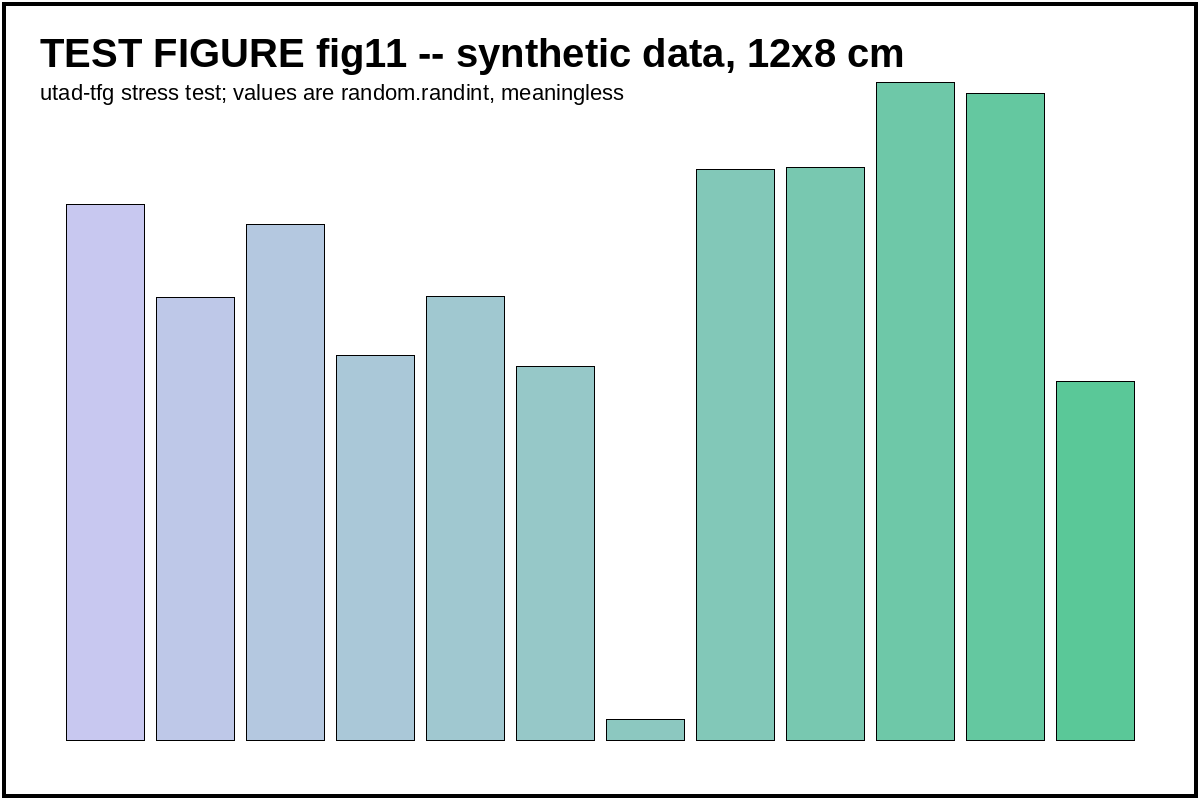
\includegraphics[width=12cm]{fig11}\caption{Fifteenth test figure. \source{Synthetic (2026)}}\end{figure}
\begin{figure}[htbp]\centering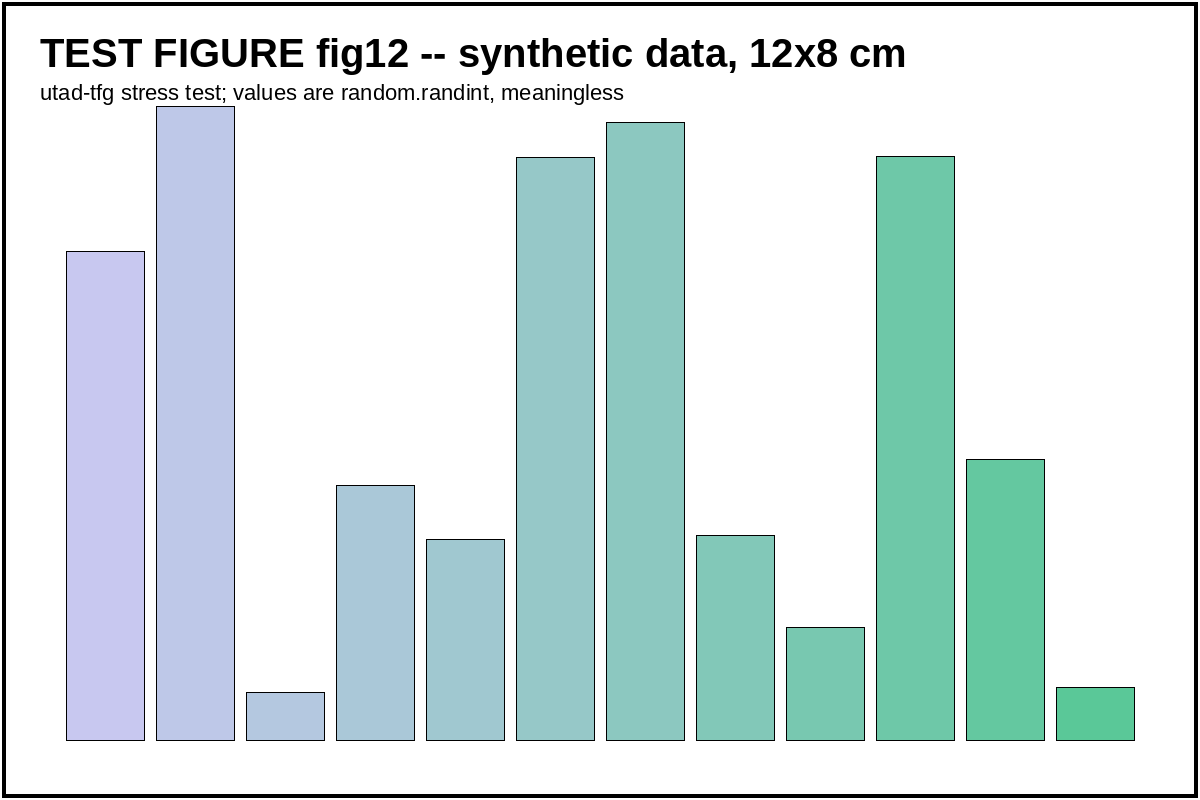
\includegraphics[width=12cm]{fig12}\caption{Sixteenth test figure. \source{Synthetic (2026)}}\end{figure}
\lipsum[78-79]
\begin{figure}[htbp]
  \centering
  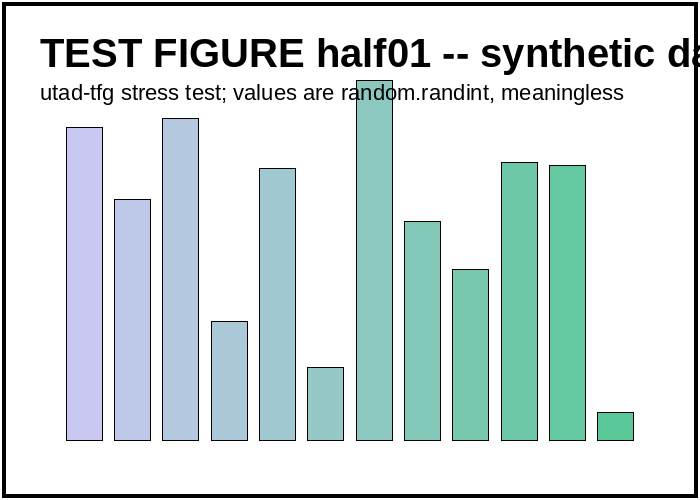
\includegraphics[width=6cm]{half01}\hfill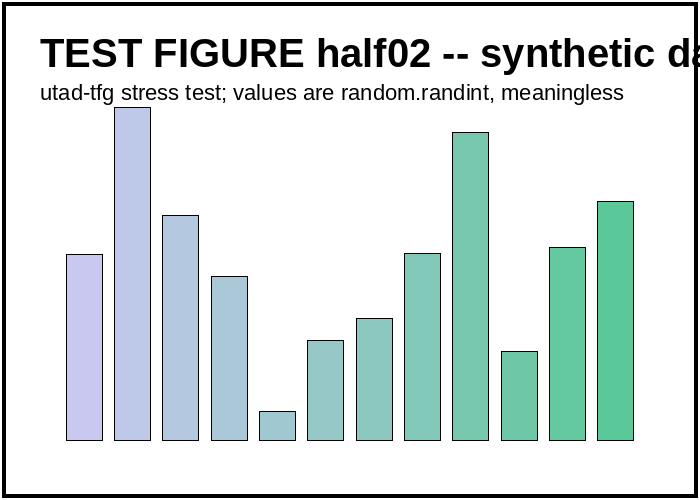
\includegraphics[width=6cm]{half02}
  \caption{Seventeenth test figure: two images side by side in one float. \source{Synthetic (2026)}}
\end{figure}
\begin{figure}[htbp]\centering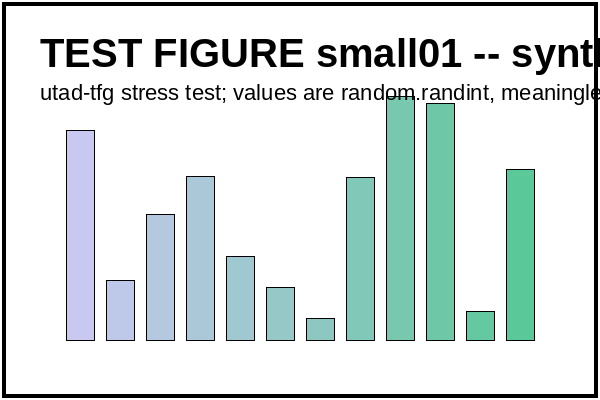
\includegraphics[width=6cm]{small01}\caption{Eighteenth test figure, small. \source{Synthetic (2026)}}\end{figure}
\begin{figure}[htbp]\centering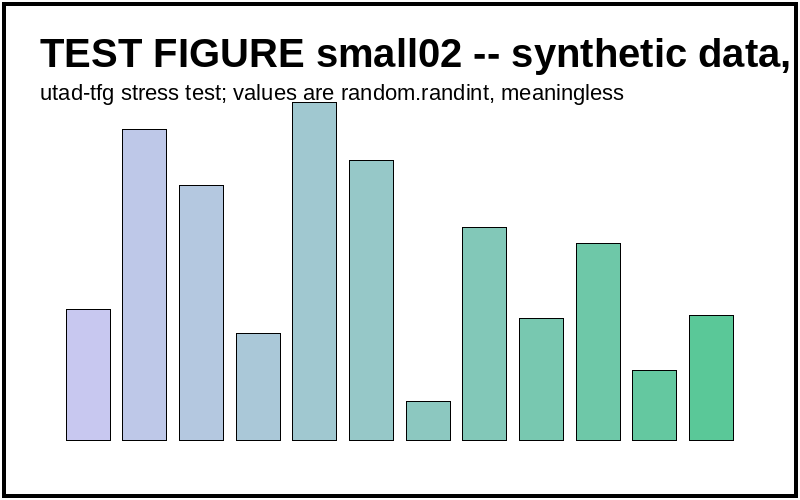
\includegraphics[width=8cm]{small02}\caption{Nineteenth test figure, small. \source{Synthetic (2026)}}\end{figure}
\lipsum[80-82]
\begin{figure}[htbp]\centering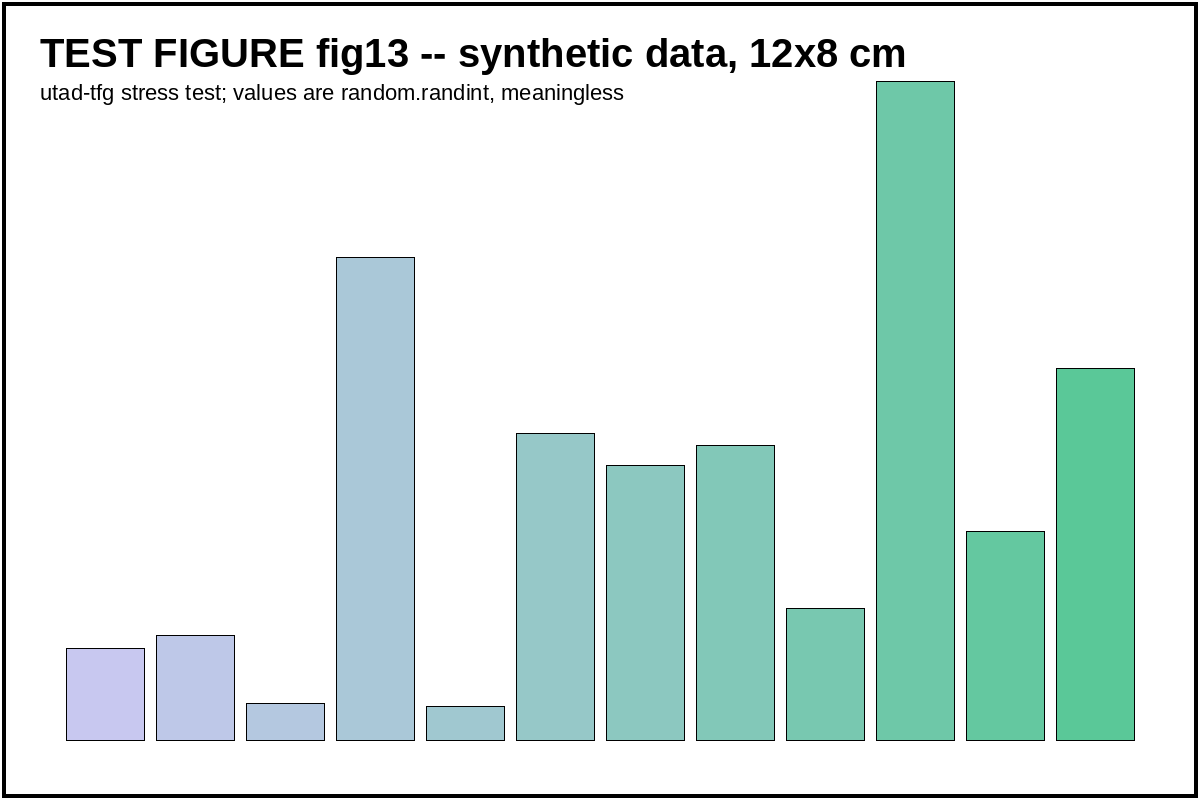
\includegraphics[width=12cm]{fig13}\caption{Twentieth test figure. \source{Synthetic (2026)}}\end{figure}
\lipsum[83-84] \parencite{ph09,ph10,ph11,ph12,ph13,ph14,ph15,ph16}.
\begin{figure}[H]\centering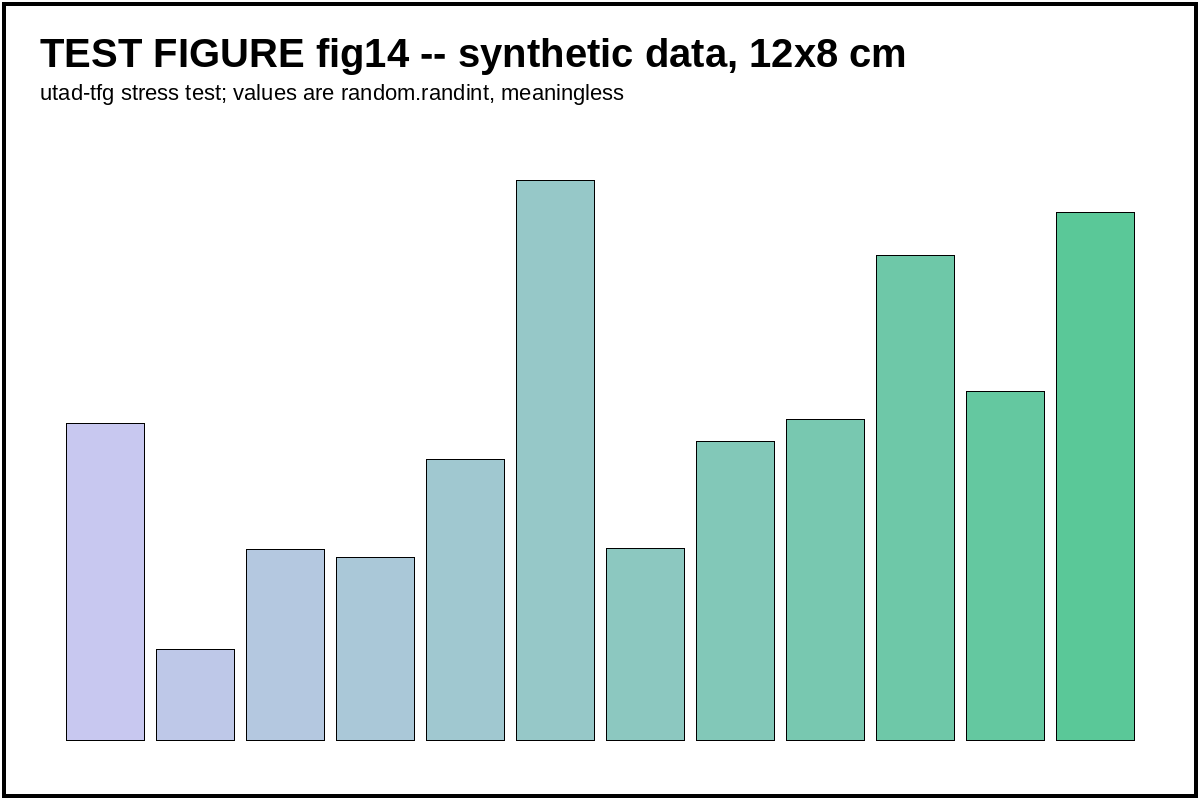
\includegraphics[width=12cm]{fig14}\caption{Twenty-first test figure, [H]. \source{Synthetic (2026)}}\end{figure}
\lipsum[85-86]
\begin{figure}[htbp]\centering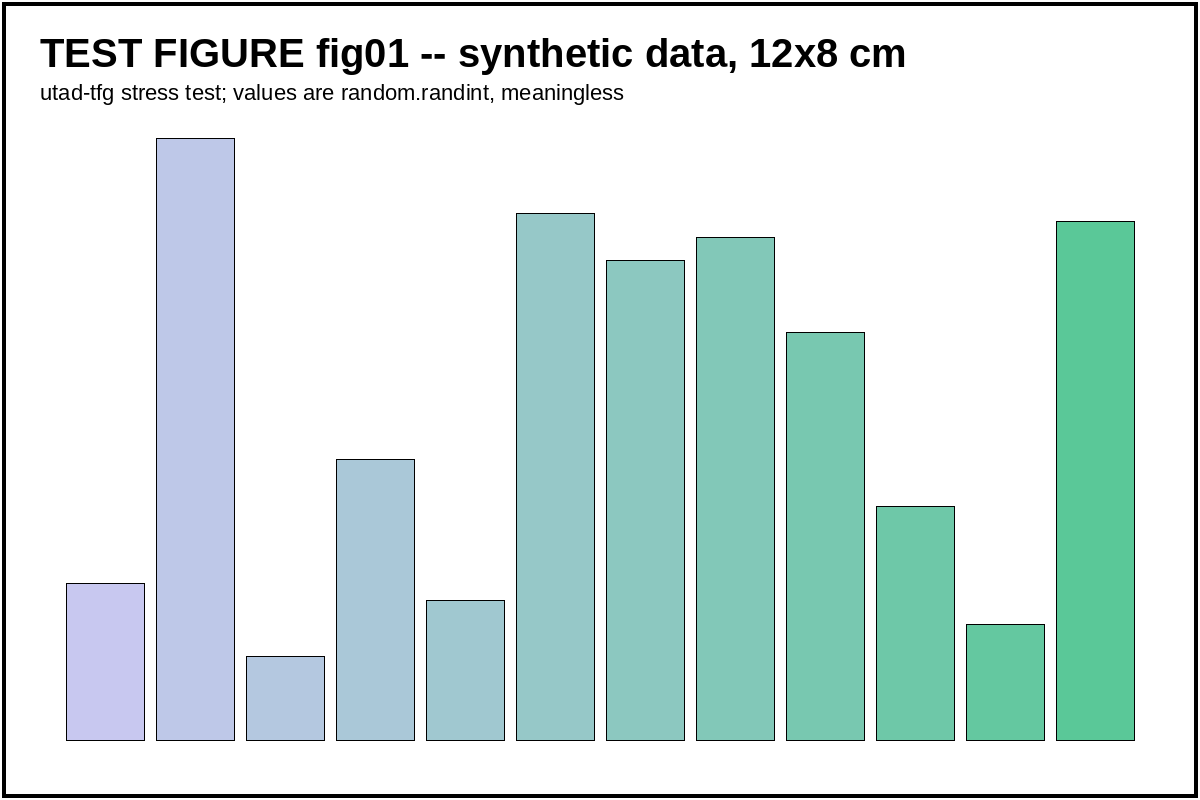
\includegraphics[width=12cm]{fig01}\caption{Twenty-second test figure, reusing the first image. \source{Synthetic (2026)}}\label{fig:last}\end{figure}

\section{Second phase}
\lipsum[87-92]
\begin{table}[htbp]
  \centering
  \caption{Sixth table. \source{Synthetic (2026)}}
  \begin{tabular}{lll}
    \toprule
    x & y & z \\
    \midrule
    1 & 2 & 3 \\
    \bottomrule
  \end{tabular}
\end{table}
\lipsum[93-98]

\section{Third phase}
\kant[6-12]

\section{Fourth phase}
\lipsum[121-135]

\section{Fifth phase}
\kant[13-20]

% =====================================================================
\chapter{Conclusions}
\lipsum[99-102] \parencite{ph17,ph18,ph19,ph20,ph21,ph22,ph23}.

\section{Discussion}
\lipsum[103-106]

\section{Further research}
\lipsum[107-109]
\lipsum[136-142]

% =====================================================================
\chapter{References}

\section{Bibliography}
\nocite{kimball2013,loshin2008,fielding2000}
\printbibliography[heading=none]

\section{Image index}
\tfgimageindex

\section{Table index}
\tfgtableindex

% =====================================================================
\begin{tfgglossary}
\begin{tfgglosslist}
\gloss{Alpha} \lipsum[110][1]
\gloss{Beta} \lipsum[110][2]
\gloss{Gamma} \lipsum[110][3]
\gloss{Delta} \lipsum[110][4]
\gloss{Epsilon} \lipsum[111][1]
\gloss{Zeta} \lipsum[111][2]
\gloss{Eta} \lipsum[111][3]
\gloss{Theta} \lipsum[111][4]
\gloss{Iota} \lipsum[112][1]
\gloss{Kappa} \lipsum[112][2]
\gloss{Lambda} \lipsum[112][3]
\gloss{Mu} \lipsum[112][4]
\end{tfgglosslist}
\end{tfgglossary}

\begin{tfgappendix}
\lipsum[113-114]

\begin{table}[H]
  \centering
  \caption{Appendix table. \source{Synthetic (2026)}}
  \begin{tabular}{lr}
    \toprule
    k & v \\
    \midrule
    a & 1 \\
    b & 2 \\
    \bottomrule
  \end{tabular}
\end{table}

\begin{lstlisting}[caption={Appendix listing.}]
placeholder = [x * x for x in range(10)]
print(placeholder)
\end{lstlisting}

\lipsum[115-120]
\end{tfgappendix}

\end{document}
